\documentclass[a4paper,17pt]{extarticle}


    \usepackage[sfdefault, condensed]{roboto} % police d'écriture plus moderne
\usepackage[french]{babel} % francisation
\usepackage[parfill]{parskip} %suppression indentation

\usepackage{fancyhdr}
\usepackage{multicol}

% figure non flotantes
\usepackage{float}
\let\origfigure\figure
\let\endorigfigure\endfigure
\renewenvironment{figure}[1][2] {
    \expandafter\origfigure\expandafter[H]
} {
    \endorigfigure
}

% mois/année
\usepackage{datetime}
\newdateformat{monthyeardate}{%
  \monthname[\THEMONTH] \THEYEAR}

% couleurs perso
\usepackage[table]{xcolor}
\definecolor{deepblue}{rgb}{0.3,0.3,0.8}
\definecolor{darkblue}{rgb}{0,0,0.3}
\definecolor{deepred}{rgb}{0.6,0,0}
\definecolor{iremred}{RGB}{204,35,50}
\definecolor{deepgreen}{rgb}{0,0.6,0}
\definecolor{backcolor}{rgb}{0.98,0.95,0.95}
\definecolor{grisClair}{rgb}{0.95,0.95,0.95}
\definecolor{orangeamu}{RGB}{250,178,11}
\definecolor{noiramu}{RGB}{35,31,32}
\definecolor{bleuamu}{RGB}{20,118,198}
\definecolor{bleuamudark}{RGB}{15,90,150}
\definecolor{cyanamu}{RGB}{77,198,244}


\usepackage{/home/bouscadilla/Documents/Code/nbconvert/template/latex/pdf_solution/xeboiboites}
%
% exemple
\newbreakabletheorem[
    small box style={fill=deepblue!90,draw=deepblue!15, rounded corners,line width=1pt},%
    big box style={fill=deepblue!5,draw=deepblue!15,thick,rounded corners,line width=1pt},%
    headfont={\color{white}\bfseries}
        ]{exemple}{Exemple}{}%{counterCo}
%
% remarque
\newbreakabletheorem[
    small box style={draw=ansi-green-intense!100,line width=2pt,fill=ansi-green-intense!0,rounded corners,decoration=penciline, decorate},%
	big box style={color=ansi-green-intense!90,fill=ansi-green-intense!10,thick,decoration={penciline},decorate},
    broken edges={draw=ansi-green-intense!90,thick,fill=orange!20!black!5, decoration={random steps, segment length=.5cm,amplitude=1.3mm},decorate},%
    other edges={decoration=penciline,decorate,thick},%
    headfont={\color{ansi-green-intense}\large\scshape\bfseries}
    ]{remarque}{Remarque}{}%{counterCa}
%
% formule (sans titre)
\newboxedequation[%
    big box style={fill=cyanamu!10,draw=cyanamu!100,thick,decoration=penciline,decorate}]%
    {form}
%
% Réponse
\newbreakabletheorem[
    small box style={fill=bleuamu!100, draw=bleuamu!60, line width=1pt,rounded corners,decorate},%
    big box style={fill=bleuamu!10,draw=bleuamu!30,thick,rounded corners,decorate},
    headfont={\color{white}\large\scshape\bfseries}
        ]{reponse}{Correction}{}
%

%
% À retenir
%\newbreakabletheorem[
%    small box style={fill=deepred!100, draw=deepred!80, line width=1pt,rounded corners,decorate},%
%    big box style={fill=deepred!10,draw=deepred!50,thick,rounded corners,decorate},
%    headfont={\color{white}\large\scshape\bfseries}
%        ]{retenir}{À retenir}{}
%
\newboxedequation[%
    big box style={fill=deepred!10,draw=deepred!0,thick,decoration=penciline,decorate}]%
    {retenir}



% astuce
\newspanning[
    image=/home/bouscadilla/Documents/Code/nbconvert/template/latex/pdf_solution/fig-idee,headfont=\bfseries,
    spanning style={very thick,decoration=penciline,decorate}
    ]{astuce}{Astuce}{}
%
% activité

\newcounter{counterCa}
\newbreakabletheorem[
    small box style={draw=orangeamu!100,line width=2pt,fill=orangeamu!100,rounded corners,decoration=penciline, decorate},%
	big box style={color=orangeamu!100,fill=orangeamu!5,thick,decoration={penciline},decorate},
    broken edges={draw=orangeamu!100,thick,fill=orangeamu!100, decoration={random steps, segment length=.5cm,amplitude=1.3mm},decorate},%
    other edges={decoration=penciline,decorate,thick},%
    headfont={\color{white}\large\scshape\bfseries}
    ]{activite}{\adjustimage{height=1cm, valign=m}{/home/bouscadilla/Documents/Code/nbconvert/template/latex/pdf_solution/papier_eleve_investigation.png}%
    Activité}{counterCa}
%   
%   environnement élève
%
\newenvironment{eleve}%
%{\begin{activite}\large\\} % écrire plus gros
{\begin{activite}\color{noiramu}\\[-0.5cm]}
{\end{activite}}

\newenvironment{formule}%
%{\begin{activite}\large\\} % écrire plus gros
{\begin{form}\color{bleuamu}}
{\end{form}}


\usepackage[breakable]{tcolorbox}
    \usepackage{parskip} % Stop auto-indenting (to mimic markdown behaviour)
    
    \usepackage{iftex}
    \ifPDFTeX
    	\usepackage[T1]{fontenc}
    	\usepackage{mathpazo}
    \else
    	\usepackage{fontspec}
    \fi

    % Basic figure setup, for now with no caption control since it's done
    % automatically by Pandoc (which extracts ![](path) syntax from Markdown).
    \usepackage{graphicx}
    % Maintain compatibility with old templates. Remove in nbconvert 6.0
    \let\Oldincludegraphics\includegraphics
    % Ensure that by default, figures have no caption (until we provide a
    % proper Figure object with a Caption API and a way to capture that
    % in the conversion process - todo).
    \usepackage{caption}
    \DeclareCaptionFormat{nocaption}{}
    \captionsetup{format=nocaption,aboveskip=0pt,belowskip=0pt}

    \usepackage[Export]{adjustbox} % Used to constrain images to a maximum size
    \adjustboxset{max size={0.9\linewidth}{0.9\paperheight}}
    \usepackage{float}
    \floatplacement{figure}{H} % forces figures to be placed at the correct location
    \usepackage{xcolor} % Allow colors to be defined
    \usepackage{enumerate} % Needed for markdown enumerations to work
    \usepackage{geometry} % Used to adjust the document margins
    \usepackage{amsmath} % Equations
    \usepackage{amssymb} % Equations
    \usepackage{textcomp} % defines textquotesingle
    % Hack from http://tex.stackexchange.com/a/47451/13684:
    \AtBeginDocument{%
        \def\PYZsq{\textquotesingle}% Upright quotes in Pygmentized code
    }
    \usepackage{upquote} % Upright quotes for verbatim code
    \usepackage{eurosym} % defines \euro
    \usepackage[mathletters]{ucs} % Extended unicode (utf-8) support
    \usepackage{fancyvrb} % verbatim replacement that allows latex

    % The hyperref package gives us a pdf with properly built
    % internal navigation ('pdf bookmarks' for the table of contents,
    % internal cross-reference links, web links for URLs, etc.)
    \usepackage{hyperref}
    % The default LaTeX title has an obnoxious amount of whitespace. By default,
    % titling removes some of it. It also provides customization options.
    \usepackage{titling}
    \usepackage{longtable} % longtable support required by pandoc >1.10
    \usepackage{booktabs}  % table support for pandoc > 1.12.2
    \usepackage[inline]{enumitem} % IRkernel/repr support (it uses the enumerate* environment)
    \usepackage[normalem]{ulem} % ulem is needed to support strikethroughs (\sout)
                                % normalem makes italics be italics, not underlines
    \usepackage{mathrsfs}
    

    
    % Colors for the hyperref package
    \definecolor{urlcolor}{rgb}{0,.145,.698}
    \definecolor{linkcolor}{rgb}{.71,0.21,0.01}
    \definecolor{citecolor}{rgb}{.12,.54,.11}

    % ANSI colors
    \definecolor{ansi-black}{HTML}{3E424D}
    \definecolor{ansi-black-intense}{HTML}{282C36}
    \definecolor{ansi-red}{HTML}{E75C58}
    \definecolor{ansi-red-intense}{HTML}{B22B31}
    \definecolor{ansi-green}{HTML}{00A250}
    \definecolor{ansi-green-intense}{HTML}{007427}
    \definecolor{ansi-yellow}{HTML}{DDB62B}
    \definecolor{ansi-yellow-intense}{HTML}{B27D12}
    \definecolor{ansi-blue}{HTML}{208FFB}
    \definecolor{ansi-blue-intense}{HTML}{0065CA}
    \definecolor{ansi-magenta}{HTML}{D160C4}
    \definecolor{ansi-magenta-intense}{HTML}{A03196}
    \definecolor{ansi-cyan}{HTML}{60C6C8}
    \definecolor{ansi-cyan-intense}{HTML}{258F8F}
    \definecolor{ansi-white}{HTML}{C5C1B4}
    \definecolor{ansi-white-intense}{HTML}{A1A6B2}
    \definecolor{ansi-default-inverse-fg}{HTML}{FFFFFF}
    \definecolor{ansi-default-inverse-bg}{HTML}{000000}

    % commands and environments needed by pandoc snippets
    % extracted from the output of `pandoc -s`
    \providecommand{\tightlist}{%
      \setlength{\itemsep}{0pt}\setlength{\parskip}{0pt}}
    \DefineVerbatimEnvironment{Highlighting}{Verbatim}{commandchars=\\\{\}}
    % Add ',fontsize=\small' for more characters per line
    \newenvironment{Shaded}{}{}
    \newcommand{\KeywordTok}[1]{\textcolor[rgb]{0.00,0.44,0.13}{\textbf{{#1}}}}
    \newcommand{\DataTypeTok}[1]{\textcolor[rgb]{0.56,0.13,0.00}{{#1}}}
    \newcommand{\DecValTok}[1]{\textcolor[rgb]{0.25,0.63,0.44}{{#1}}}
    \newcommand{\BaseNTok}[1]{\textcolor[rgb]{0.25,0.63,0.44}{{#1}}}
    \newcommand{\FloatTok}[1]{\textcolor[rgb]{0.25,0.63,0.44}{{#1}}}
    \newcommand{\CharTok}[1]{\textcolor[rgb]{0.25,0.44,0.63}{{#1}}}
    \newcommand{\StringTok}[1]{\textcolor[rgb]{0.25,0.44,0.63}{{#1}}}
    \newcommand{\CommentTok}[1]{\textcolor[rgb]{0.38,0.63,0.69}{\textit{{#1}}}}
    \newcommand{\OtherTok}[1]{\textcolor[rgb]{0.00,0.44,0.13}{{#1}}}
    \newcommand{\AlertTok}[1]{\textcolor[rgb]{1.00,0.00,0.00}{\textbf{{#1}}}}
    \newcommand{\FunctionTok}[1]{\textcolor[rgb]{0.02,0.16,0.49}{{#1}}}
    \newcommand{\RegionMarkerTok}[1]{{#1}}
    \newcommand{\ErrorTok}[1]{\textcolor[rgb]{1.00,0.00,0.00}{\textbf{{#1}}}}
    \newcommand{\NormalTok}[1]{{#1}}
    
    % Additional commands for more recent versions of Pandoc
    \newcommand{\ConstantTok}[1]{\textcolor[rgb]{0.53,0.00,0.00}{{#1}}}
    \newcommand{\SpecialCharTok}[1]{\textcolor[rgb]{0.25,0.44,0.63}{{#1}}}
    \newcommand{\VerbatimStringTok}[1]{\textcolor[rgb]{0.25,0.44,0.63}{{#1}}}
    \newcommand{\SpecialStringTok}[1]{\textcolor[rgb]{0.73,0.40,0.53}{{#1}}}
    \newcommand{\ImportTok}[1]{{#1}}
    \newcommand{\DocumentationTok}[1]{\textcolor[rgb]{0.73,0.13,0.13}{\textit{{#1}}}}
    \newcommand{\AnnotationTok}[1]{\textcolor[rgb]{0.38,0.63,0.69}{\textbf{\textit{{#1}}}}}
    \newcommand{\CommentVarTok}[1]{\textcolor[rgb]{0.38,0.63,0.69}{\textbf{\textit{{#1}}}}}
    \newcommand{\VariableTok}[1]{\textcolor[rgb]{0.10,0.09,0.49}{{#1}}}
    \newcommand{\ControlFlowTok}[1]{\textcolor[rgb]{0.00,0.44,0.13}{\textbf{{#1}}}}
    \newcommand{\OperatorTok}[1]{\textcolor[rgb]{0.40,0.40,0.40}{{#1}}}
    \newcommand{\BuiltInTok}[1]{{#1}}
    \newcommand{\ExtensionTok}[1]{{#1}}
    \newcommand{\PreprocessorTok}[1]{\textcolor[rgb]{0.74,0.48,0.00}{{#1}}}
    \newcommand{\AttributeTok}[1]{\textcolor[rgb]{0.49,0.56,0.16}{{#1}}}
    \newcommand{\InformationTok}[1]{\textcolor[rgb]{0.38,0.63,0.69}{\textbf{\textit{{#1}}}}}
    \newcommand{\WarningTok}[1]{\textcolor[rgb]{0.38,0.63,0.69}{\textbf{\textit{{#1}}}}}
    
    
    % Define a nice break command that doesn't care if a line doesn't already
    % exist.
    \def\br{\hspace*{\fill} \\* }
    % Math Jax compatibility definitions
    \def\gt{>}
    \def\lt{<}
    \let\Oldtex\TeX
    \let\Oldlatex\LaTeX
    \renewcommand{\TeX}{\textrm{\Oldtex}}
    \renewcommand{\LaTeX}{\textrm{\Oldlatex}}
    % Document parameters
    % Document title
    \title{5-3---ListesChainees-operations}
    
    
    
    
    
% Pygments definitions
\makeatletter
\def\PY@reset{\let\PY@it=\relax \let\PY@bf=\relax%
    \let\PY@ul=\relax \let\PY@tc=\relax%
    \let\PY@bc=\relax \let\PY@ff=\relax}
\def\PY@tok#1{\csname PY@tok@#1\endcsname}
\def\PY@toks#1+{\ifx\relax#1\empty\else%
    \PY@tok{#1}\expandafter\PY@toks\fi}
\def\PY@do#1{\PY@bc{\PY@tc{\PY@ul{%
    \PY@it{\PY@bf{\PY@ff{#1}}}}}}}
\def\PY#1#2{\PY@reset\PY@toks#1+\relax+\PY@do{#2}}

\expandafter\def\csname PY@tok@w\endcsname{\def\PY@tc##1{\textcolor[rgb]{0.73,0.73,0.73}{##1}}}
\expandafter\def\csname PY@tok@c\endcsname{\let\PY@it=\textit\def\PY@tc##1{\textcolor[rgb]{0.25,0.50,0.50}{##1}}}
\expandafter\def\csname PY@tok@cp\endcsname{\def\PY@tc##1{\textcolor[rgb]{0.74,0.48,0.00}{##1}}}
\expandafter\def\csname PY@tok@k\endcsname{\let\PY@bf=\textbf\def\PY@tc##1{\textcolor[rgb]{0.00,0.50,0.00}{##1}}}
\expandafter\def\csname PY@tok@kp\endcsname{\def\PY@tc##1{\textcolor[rgb]{0.00,0.50,0.00}{##1}}}
\expandafter\def\csname PY@tok@kt\endcsname{\def\PY@tc##1{\textcolor[rgb]{0.69,0.00,0.25}{##1}}}
\expandafter\def\csname PY@tok@o\endcsname{\def\PY@tc##1{\textcolor[rgb]{0.40,0.40,0.40}{##1}}}
\expandafter\def\csname PY@tok@ow\endcsname{\let\PY@bf=\textbf\def\PY@tc##1{\textcolor[rgb]{0.67,0.13,1.00}{##1}}}
\expandafter\def\csname PY@tok@nb\endcsname{\def\PY@tc##1{\textcolor[rgb]{0.00,0.50,0.00}{##1}}}
\expandafter\def\csname PY@tok@nf\endcsname{\def\PY@tc##1{\textcolor[rgb]{0.00,0.00,1.00}{##1}}}
\expandafter\def\csname PY@tok@nc\endcsname{\let\PY@bf=\textbf\def\PY@tc##1{\textcolor[rgb]{0.00,0.00,1.00}{##1}}}
\expandafter\def\csname PY@tok@nn\endcsname{\let\PY@bf=\textbf\def\PY@tc##1{\textcolor[rgb]{0.00,0.00,1.00}{##1}}}
\expandafter\def\csname PY@tok@ne\endcsname{\let\PY@bf=\textbf\def\PY@tc##1{\textcolor[rgb]{0.82,0.25,0.23}{##1}}}
\expandafter\def\csname PY@tok@nv\endcsname{\def\PY@tc##1{\textcolor[rgb]{0.10,0.09,0.49}{##1}}}
\expandafter\def\csname PY@tok@no\endcsname{\def\PY@tc##1{\textcolor[rgb]{0.53,0.00,0.00}{##1}}}
\expandafter\def\csname PY@tok@nl\endcsname{\def\PY@tc##1{\textcolor[rgb]{0.63,0.63,0.00}{##1}}}
\expandafter\def\csname PY@tok@ni\endcsname{\let\PY@bf=\textbf\def\PY@tc##1{\textcolor[rgb]{0.60,0.60,0.60}{##1}}}
\expandafter\def\csname PY@tok@na\endcsname{\def\PY@tc##1{\textcolor[rgb]{0.49,0.56,0.16}{##1}}}
\expandafter\def\csname PY@tok@nt\endcsname{\let\PY@bf=\textbf\def\PY@tc##1{\textcolor[rgb]{0.00,0.50,0.00}{##1}}}
\expandafter\def\csname PY@tok@nd\endcsname{\def\PY@tc##1{\textcolor[rgb]{0.67,0.13,1.00}{##1}}}
\expandafter\def\csname PY@tok@s\endcsname{\def\PY@tc##1{\textcolor[rgb]{0.73,0.13,0.13}{##1}}}
\expandafter\def\csname PY@tok@sd\endcsname{\let\PY@it=\textit\def\PY@tc##1{\textcolor[rgb]{0.73,0.13,0.13}{##1}}}
\expandafter\def\csname PY@tok@si\endcsname{\let\PY@bf=\textbf\def\PY@tc##1{\textcolor[rgb]{0.73,0.40,0.53}{##1}}}
\expandafter\def\csname PY@tok@se\endcsname{\let\PY@bf=\textbf\def\PY@tc##1{\textcolor[rgb]{0.73,0.40,0.13}{##1}}}
\expandafter\def\csname PY@tok@sr\endcsname{\def\PY@tc##1{\textcolor[rgb]{0.73,0.40,0.53}{##1}}}
\expandafter\def\csname PY@tok@ss\endcsname{\def\PY@tc##1{\textcolor[rgb]{0.10,0.09,0.49}{##1}}}
\expandafter\def\csname PY@tok@sx\endcsname{\def\PY@tc##1{\textcolor[rgb]{0.00,0.50,0.00}{##1}}}
\expandafter\def\csname PY@tok@m\endcsname{\def\PY@tc##1{\textcolor[rgb]{0.40,0.40,0.40}{##1}}}
\expandafter\def\csname PY@tok@gh\endcsname{\let\PY@bf=\textbf\def\PY@tc##1{\textcolor[rgb]{0.00,0.00,0.50}{##1}}}
\expandafter\def\csname PY@tok@gu\endcsname{\let\PY@bf=\textbf\def\PY@tc##1{\textcolor[rgb]{0.50,0.00,0.50}{##1}}}
\expandafter\def\csname PY@tok@gd\endcsname{\def\PY@tc##1{\textcolor[rgb]{0.63,0.00,0.00}{##1}}}
\expandafter\def\csname PY@tok@gi\endcsname{\def\PY@tc##1{\textcolor[rgb]{0.00,0.63,0.00}{##1}}}
\expandafter\def\csname PY@tok@gr\endcsname{\def\PY@tc##1{\textcolor[rgb]{1.00,0.00,0.00}{##1}}}
\expandafter\def\csname PY@tok@ge\endcsname{\let\PY@it=\textit}
\expandafter\def\csname PY@tok@gs\endcsname{\let\PY@bf=\textbf}
\expandafter\def\csname PY@tok@gp\endcsname{\let\PY@bf=\textbf\def\PY@tc##1{\textcolor[rgb]{0.00,0.00,0.50}{##1}}}
\expandafter\def\csname PY@tok@go\endcsname{\def\PY@tc##1{\textcolor[rgb]{0.53,0.53,0.53}{##1}}}
\expandafter\def\csname PY@tok@gt\endcsname{\def\PY@tc##1{\textcolor[rgb]{0.00,0.27,0.87}{##1}}}
\expandafter\def\csname PY@tok@err\endcsname{\def\PY@bc##1{\setlength{\fboxsep}{0pt}\fcolorbox[rgb]{1.00,0.00,0.00}{1,1,1}{\strut ##1}}}
\expandafter\def\csname PY@tok@kc\endcsname{\let\PY@bf=\textbf\def\PY@tc##1{\textcolor[rgb]{0.00,0.50,0.00}{##1}}}
\expandafter\def\csname PY@tok@kd\endcsname{\let\PY@bf=\textbf\def\PY@tc##1{\textcolor[rgb]{0.00,0.50,0.00}{##1}}}
\expandafter\def\csname PY@tok@kn\endcsname{\let\PY@bf=\textbf\def\PY@tc##1{\textcolor[rgb]{0.00,0.50,0.00}{##1}}}
\expandafter\def\csname PY@tok@kr\endcsname{\let\PY@bf=\textbf\def\PY@tc##1{\textcolor[rgb]{0.00,0.50,0.00}{##1}}}
\expandafter\def\csname PY@tok@bp\endcsname{\def\PY@tc##1{\textcolor[rgb]{0.00,0.50,0.00}{##1}}}
\expandafter\def\csname PY@tok@fm\endcsname{\def\PY@tc##1{\textcolor[rgb]{0.00,0.00,1.00}{##1}}}
\expandafter\def\csname PY@tok@vc\endcsname{\def\PY@tc##1{\textcolor[rgb]{0.10,0.09,0.49}{##1}}}
\expandafter\def\csname PY@tok@vg\endcsname{\def\PY@tc##1{\textcolor[rgb]{0.10,0.09,0.49}{##1}}}
\expandafter\def\csname PY@tok@vi\endcsname{\def\PY@tc##1{\textcolor[rgb]{0.10,0.09,0.49}{##1}}}
\expandafter\def\csname PY@tok@vm\endcsname{\def\PY@tc##1{\textcolor[rgb]{0.10,0.09,0.49}{##1}}}
\expandafter\def\csname PY@tok@sa\endcsname{\def\PY@tc##1{\textcolor[rgb]{0.73,0.13,0.13}{##1}}}
\expandafter\def\csname PY@tok@sb\endcsname{\def\PY@tc##1{\textcolor[rgb]{0.73,0.13,0.13}{##1}}}
\expandafter\def\csname PY@tok@sc\endcsname{\def\PY@tc##1{\textcolor[rgb]{0.73,0.13,0.13}{##1}}}
\expandafter\def\csname PY@tok@dl\endcsname{\def\PY@tc##1{\textcolor[rgb]{0.73,0.13,0.13}{##1}}}
\expandafter\def\csname PY@tok@s2\endcsname{\def\PY@tc##1{\textcolor[rgb]{0.73,0.13,0.13}{##1}}}
\expandafter\def\csname PY@tok@sh\endcsname{\def\PY@tc##1{\textcolor[rgb]{0.73,0.13,0.13}{##1}}}
\expandafter\def\csname PY@tok@s1\endcsname{\def\PY@tc##1{\textcolor[rgb]{0.73,0.13,0.13}{##1}}}
\expandafter\def\csname PY@tok@mb\endcsname{\def\PY@tc##1{\textcolor[rgb]{0.40,0.40,0.40}{##1}}}
\expandafter\def\csname PY@tok@mf\endcsname{\def\PY@tc##1{\textcolor[rgb]{0.40,0.40,0.40}{##1}}}
\expandafter\def\csname PY@tok@mh\endcsname{\def\PY@tc##1{\textcolor[rgb]{0.40,0.40,0.40}{##1}}}
\expandafter\def\csname PY@tok@mi\endcsname{\def\PY@tc##1{\textcolor[rgb]{0.40,0.40,0.40}{##1}}}
\expandafter\def\csname PY@tok@il\endcsname{\def\PY@tc##1{\textcolor[rgb]{0.40,0.40,0.40}{##1}}}
\expandafter\def\csname PY@tok@mo\endcsname{\def\PY@tc##1{\textcolor[rgb]{0.40,0.40,0.40}{##1}}}
\expandafter\def\csname PY@tok@ch\endcsname{\let\PY@it=\textit\def\PY@tc##1{\textcolor[rgb]{0.25,0.50,0.50}{##1}}}
\expandafter\def\csname PY@tok@cm\endcsname{\let\PY@it=\textit\def\PY@tc##1{\textcolor[rgb]{0.25,0.50,0.50}{##1}}}
\expandafter\def\csname PY@tok@cpf\endcsname{\let\PY@it=\textit\def\PY@tc##1{\textcolor[rgb]{0.25,0.50,0.50}{##1}}}
\expandafter\def\csname PY@tok@c1\endcsname{\let\PY@it=\textit\def\PY@tc##1{\textcolor[rgb]{0.25,0.50,0.50}{##1}}}
\expandafter\def\csname PY@tok@cs\endcsname{\let\PY@it=\textit\def\PY@tc##1{\textcolor[rgb]{0.25,0.50,0.50}{##1}}}

\def\PYZbs{\char`\\}
\def\PYZus{\char`\_}
\def\PYZob{\char`\{}
\def\PYZcb{\char`\}}
\def\PYZca{\char`\^}
\def\PYZam{\char`\&}
\def\PYZlt{\char`\<}
\def\PYZgt{\char`\>}
\def\PYZsh{\char`\#}
\def\PYZpc{\char`\%}
\def\PYZdl{\char`\$}
\def\PYZhy{\char`\-}
\def\PYZsq{\char`\'}
\def\PYZdq{\char`\"}
\def\PYZti{\char`\~}
% for compatibility with earlier versions
\def\PYZat{@}
\def\PYZlb{[}
\def\PYZrb{]}
\makeatother


    % For linebreaks inside Verbatim environment from package fancyvrb. 
    \makeatletter
        \newbox\Wrappedcontinuationbox 
        \newbox\Wrappedvisiblespacebox 
        \newcommand*\Wrappedvisiblespace {\textcolor{red}{\textvisiblespace}} 
        \newcommand*\Wrappedcontinuationsymbol {\textcolor{red}{\llap{\tiny$\m@th\hookrightarrow$}}} 
        \newcommand*\Wrappedcontinuationindent {3ex } 
        \newcommand*\Wrappedafterbreak {\kern\Wrappedcontinuationindent\copy\Wrappedcontinuationbox} 
        % Take advantage of the already applied Pygments mark-up to insert 
        % potential linebreaks for TeX processing. 
        %        {, <, #, %, $, ' and ": go to next line. 
        %        _, }, ^, &, >, - and ~: stay at end of broken line. 
        % Use of \textquotesingle for straight quote. 
        \newcommand*\Wrappedbreaksatspecials {% 
            \def\PYGZus{\discretionary{\char`\_}{\Wrappedafterbreak}{\char`\_}}% 
            \def\PYGZob{\discretionary{}{\Wrappedafterbreak\char`\{}{\char`\{}}% 
            \def\PYGZcb{\discretionary{\char`\}}{\Wrappedafterbreak}{\char`\}}}% 
            \def\PYGZca{\discretionary{\char`\^}{\Wrappedafterbreak}{\char`\^}}% 
            \def\PYGZam{\discretionary{\char`\&}{\Wrappedafterbreak}{\char`\&}}% 
            \def\PYGZlt{\discretionary{}{\Wrappedafterbreak\char`\<}{\char`\<}}% 
            \def\PYGZgt{\discretionary{\char`\>}{\Wrappedafterbreak}{\char`\>}}% 
            \def\PYGZsh{\discretionary{}{\Wrappedafterbreak\char`\#}{\char`\#}}% 
            \def\PYGZpc{\discretionary{}{\Wrappedafterbreak\char`\%}{\char`\%}}% 
            \def\PYGZdl{\discretionary{}{\Wrappedafterbreak\char`\$}{\char`\$}}% 
            \def\PYGZhy{\discretionary{\char`\-}{\Wrappedafterbreak}{\char`\-}}% 
            \def\PYGZsq{\discretionary{}{\Wrappedafterbreak\textquotesingle}{\textquotesingle}}% 
            \def\PYGZdq{\discretionary{}{\Wrappedafterbreak\char`\"}{\char`\"}}% 
            \def\PYGZti{\discretionary{\char`\~}{\Wrappedafterbreak}{\char`\~}}% 
        } 
        % Some characters . , ; ? ! / are not pygmentized. 
        % This macro makes them "active" and they will insert potential linebreaks 
        \newcommand*\Wrappedbreaksatpunct {% 
            \lccode`\~`\.\lowercase{\def~}{\discretionary{\hbox{\char`\.}}{\Wrappedafterbreak}{\hbox{\char`\.}}}% 
            \lccode`\~`\,\lowercase{\def~}{\discretionary{\hbox{\char`\,}}{\Wrappedafterbreak}{\hbox{\char`\,}}}% 
            \lccode`\~`\;\lowercase{\def~}{\discretionary{\hbox{\char`\;}}{\Wrappedafterbreak}{\hbox{\char`\;}}}% 
            \lccode`\~`\:\lowercase{\def~}{\discretionary{\hbox{\char`\:}}{\Wrappedafterbreak}{\hbox{\char`\:}}}% 
            \lccode`\~`\?\lowercase{\def~}{\discretionary{\hbox{\char`\?}}{\Wrappedafterbreak}{\hbox{\char`\?}}}% 
            \lccode`\~`\!\lowercase{\def~}{\discretionary{\hbox{\char`\!}}{\Wrappedafterbreak}{\hbox{\char`\!}}}% 
            \lccode`\~`\/\lowercase{\def~}{\discretionary{\hbox{\char`\/}}{\Wrappedafterbreak}{\hbox{\char`\/}}}% 
            \catcode`\.\active
            \catcode`\,\active 
            \catcode`\;\active
            \catcode`\:\active
            \catcode`\?\active
            \catcode`\!\active
            \catcode`\/\active 
            \lccode`\~`\~ 	
        }
    \makeatother

    \let\OriginalVerbatim=\Verbatim
    \makeatletter
    \renewcommand{\Verbatim}[1][1]{%
        %\parskip\z@skip
        \sbox\Wrappedcontinuationbox {\Wrappedcontinuationsymbol}%
        \sbox\Wrappedvisiblespacebox {\FV@SetupFont\Wrappedvisiblespace}%
        \def\FancyVerbFormatLine ##1{\hsize\linewidth
            \vtop{\raggedright\hyphenpenalty\z@\exhyphenpenalty\z@
                \doublehyphendemerits\z@\finalhyphendemerits\z@
                \strut ##1\strut}%
        }%
        % If the linebreak is at a space, the latter will be displayed as visible
        % space at end of first line, and a continuation symbol starts next line.
        % Stretch/shrink are however usually zero for typewriter font.
        \def\FV@Space {%
            \nobreak\hskip\z@ plus\fontdimen3\font minus\fontdimen4\font
            \discretionary{\copy\Wrappedvisiblespacebox}{\Wrappedafterbreak}
            {\kern\fontdimen2\font}%
        }%
        
        % Allow breaks at special characters using \PYG... macros.
        \Wrappedbreaksatspecials
        % Breaks at punctuation characters . , ; ? ! and / need catcode=\active 	
        \OriginalVerbatim[#1,codes*=\Wrappedbreaksatpunct]%
    }
    \makeatother

    % Exact colors from NB
    \definecolor{incolor}{HTML}{303F9F}
    \definecolor{outcolor}{HTML}{D84315}
    \definecolor{cellborder}{HTML}{CFCFCF}
    \definecolor{cellbackground}{HTML}{F7F7F7}
    
    % prompt
    \makeatletter
    \newcommand{\boxspacing}{\kern\kvtcb@left@rule\kern\kvtcb@boxsep}
    \makeatother
    \newcommand{\prompt}[4]{
        \ttfamily\llap{{\color{#2}[#3]:\hspace{3pt}#4}}\vspace{-\baselineskip}
    }
    

    
\setlength\headheight{30pt}
\setcounter{secnumdepth}{0} % Turns off numbering for sections

    % Prevent overflowing lines due to hard-to-break entities
    \sloppy 
    % Setup hyperref package
    \hypersetup{
      breaklinks=true,  % so long urls are correctly broken across lines
      colorlinks=true,
      urlcolor=urlcolor,
      linkcolor=linkcolor,
      citecolor=citecolor,
      }
    % Slightly bigger margins than the latex defaults
    \geometry{a4paper,tmargin=3cm,bmargin=2cm,lmargin=1cm,rmargin=1cm}\fancyhead[L]{Thème à définir}\fancyhead[L]{\adjustimage{height=1cm, valign=m}{/home/bouscadilla/Documents/Code/nbconvert/template/latex/pdf_solution/papier_eleve_ico_structure}\ttfamily\scshape Struct.de données}\fancyhead[C]{\bfseries\MakeUppercase{5-3---ListesChainees-operations}}\fancyhead[C]{\bfseries\MakeUppercase{5 --- Listes chaînées}}\fancyhead[R]{\monthyeardate\today}

    \fancyfoot[C]{\thepage}
    % #TODO ajouter les pages totales

    \pagestyle{fancy}
    


\begin{document}
    
    \title{5 --- Listes chaînées}
% \maketitle

    
    

    
    \hypertarget{opuxe9rations-sur-les-listes}{%
\subsection{3 --- Opérations sur les
listes}\label{opuxe9rations-sur-les-listes}}

    Comme on l'a vu dans la partie 2, on se munit pour la suite d'une classe
\texttt{Maillon} possède deux attributs : \texttt{valeur} et
\texttt{suivant}.

        {\scriptsize
    \begin{tcolorbox}[breakable, size=fbox, boxrule=1pt, pad at break*=1mm,colback=cellbackground, colframe=cellborder]
\prompt{In}{incolor}{1}{\boxspacing}
\begin{Verbatim}[commandchars=\\\{\}]
\PY{k+kn}{from} \PY{n+nn}{doctest} \PY{k+kn}{import} \PY{n}{testmod}
\end{Verbatim}
\end{tcolorbox}
    }

        {\scriptsize
    \begin{tcolorbox}[breakable, size=fbox, boxrule=1pt, pad at break*=1mm,colback=cellbackground, colframe=cellborder]
\prompt{In}{incolor}{2}{\boxspacing}
\begin{Verbatim}[commandchars=\\\{\}]
\PY{k}{class} \PY{n+nc}{Maillon}\PY{p}{:}
    \PY{l+s+sd}{\PYZdq{}\PYZdq{}\PYZdq{}}
\PY{l+s+sd}{    Une classe pour représenter le maillon d\PYZsq{}une liste}

\PY{l+s+sd}{    Attributs}
\PY{l+s+sd}{    \PYZhy{}\PYZhy{}\PYZhy{}\PYZhy{}\PYZhy{}\PYZhy{}\PYZhy{}\PYZhy{}\PYZhy{}}
\PY{l+s+sd}{    valeur : type}
\PY{l+s+sd}{        valeur contenue dans le maillon}
\PY{l+s+sd}{    suivant : maillon}
\PY{l+s+sd}{        maillon suivant ou None si pas de maillon}
\PY{l+s+sd}{    \PYZdq{}\PYZdq{}\PYZdq{}}

    \PY{k}{def} \PY{n+nf+fm}{\PYZus{}\PYZus{}init\PYZus{}\PYZus{}}\PY{p}{(}\PY{n+nb+bp}{self}\PY{p}{,} \PY{n}{valeur}\PY{p}{,} \PY{n}{suivant}\PY{p}{)}\PY{p}{:}
        \PY{l+s+sd}{\PYZdq{}\PYZdq{}\PYZdq{}Constructeur de classe}

\PY{l+s+sd}{        Args:}
\PY{l+s+sd}{            valeur (type): valeur stockée dans le maillon}
\PY{l+s+sd}{            suivant (maillon): maillon suivant ou None}

\PY{l+s+sd}{        Exemples et tests:}
\PY{l+s+sd}{        \PYZgt{}\PYZgt{}\PYZgt{} l3 = Maillon(3, None)}
\PY{l+s+sd}{        \PYZgt{}\PYZgt{}\PYZgt{} assert (l3.valeur == 3)}
\PY{l+s+sd}{        \PYZgt{}\PYZgt{}\PYZgt{} assert (l3.suivant == None)}
\PY{l+s+sd}{        }
\PY{l+s+sd}{        \PYZgt{}\PYZgt{}\PYZgt{} l2 = Maillon(2, l3)}
\PY{l+s+sd}{        \PYZgt{}\PYZgt{}\PYZgt{} assert (l2.valeur == 2)}
\PY{l+s+sd}{        \PYZgt{}\PYZgt{}\PYZgt{} assert (l2.suivant.valeur == 3)}

\PY{l+s+sd}{        \PYZgt{}\PYZgt{}\PYZgt{} l1 = Maillon(1, l2)}
\PY{l+s+sd}{        \PYZgt{}\PYZgt{}\PYZgt{} assert (l1.valeur == 1)}
\PY{l+s+sd}{        \PYZgt{}\PYZgt{}\PYZgt{} assert (l1.suivant.valeur == 2)}
\PY{l+s+sd}{        \PYZgt{}\PYZgt{}\PYZgt{} assert (l1.suivant.suivant.valeur == 3)}
\PY{l+s+sd}{        \PYZgt{}\PYZgt{}\PYZgt{} assert (l1.suivant.suivant.suivant == None)}
\PY{l+s+sd}{        }
\PY{l+s+sd}{        \PYZgt{}\PYZgt{}\PYZgt{} l1.suivant.suivant.suivant.valeur}
\PY{l+s+sd}{        Traceback (most recent call last):}
\PY{l+s+sd}{        AttributeError: \PYZsq{}NoneType\PYZsq{} object has no attribute \PYZsq{}valeur\PYZsq{}}
\PY{l+s+sd}{        \PYZdq{}\PYZdq{}\PYZdq{}}
        \PY{n+nb+bp}{self}\PY{o}{.}\PY{n}{valeur} \PY{o}{=} \PY{n}{valeur}
        \PY{n+nb+bp}{self}\PY{o}{.}\PY{n}{suivant} \PY{o}{=} \PY{n}{suivant}


\PY{n}{testmod}\PY{p}{(}\PY{p}{)}
\end{Verbatim}
\end{tcolorbox}
    }

            \begin{tcolorbox}[breakable, size=fbox, boxrule=.5pt, pad at break*=1mm, opacityfill=0]
\prompt{Out}{outcolor}{2}{\boxspacing}
\begin{Verbatim}[commandchars=\\\{\}]
TestResults(failed=0, attempted=12)
\end{Verbatim}
\end{tcolorbox}
        
    \hypertarget{longueur-dune-liste}{%
\subsubsection{3.1 --- Longueur d'une liste}\label{longueur-dune-liste}}

    \hypertarget{par-une-fonction-ruxe9cursive}{%
\paragraph{Par une fonction
récursive}\label{par-une-fonction-ruxe9cursive}}

    L'objectif est d'implémenter une fonction récursive \texttt{longueur}
qui reçoit en argument une liste \texttt{lst} et renvoie sa longueur.

Il faut distinguer le \textbf{cas de base} (c'est-à-dire une liste vide
ne contenant aucun maillon) et le \textbf{cas récursif} c'est-à-dire une
liste contenant au moins un maillon.

\begin{enumerate}
\def\labelenumi{\arabic{enumi}.}
\tightlist
\item
  pour le cas de base, il faut renvoyer \texttt{0} car c'est une liste
  de longueur nulle ;
\item
  pour le cas récursif, il faut renvoyer la somme de \texttt{1} (pour le
  premier maillon) avec la longueur de la liste \texttt{lst.suivant}
  (que l'on calcule récursivement)
\end{enumerate}
\begin{eleve}
    \textbf{Implémenter la fonction récursive
\texttt{longueur(lst)\ -\textgreater{}\ int} qui renvoie la longueur de
la liste \texttt{lst}.}

\emph{Exemple 1 : l'instruction
\texttt{print(\ longueur(Maillon(42,\ None))\ )} doit afficher
\texttt{1} car cette liste ne contient qu'un seul maillon.} :

\begin{verbatim}
    >>> print( longueur(Maillon(42, None)) )
    1
\end{verbatim}

\emph{Exemple 2 : l'instruction \texttt{print(\ longueur(None)\ )} doit
afficher \texttt{0} car c'est la liste vide.}

\begin{verbatim}
    >>> print( longueur(None) )
    0
\end{verbatim}

\emph{Exemple 3 : l'instruction
\texttt{print(longueur(\ Maillon(1,\ Maillon(2,\ Maillon(3,\ None)))\ ))}
doit afficher \texttt{3}.}

\begin{verbatim}
    >>> print(longueur( Maillon(1, Maillon(2, Maillon(3, None))) ))
    3
\end{verbatim}
        
        \end{eleve}\begin{reponse}
        {\scriptsize
    \begin{tcolorbox}[breakable, size=fbox, boxrule=1pt, pad at break*=1mm,colback=cellbackground, colframe=cellborder]
\prompt{In}{incolor}{3}{\boxspacing}
\begin{Verbatim}[commandchars=\\\{\}]
\PY{k}{def} \PY{n+nf}{longueur}\PY{p}{(}\PY{n}{lst}\PY{p}{)}\PY{p}{:}
    \PY{l+s+sd}{\PYZdq{}\PYZdq{}\PYZdq{} longueur d\PYZsq{}une liste chaînée}
\PY{l+s+sd}{    }
\PY{l+s+sd}{    Exemples et tests:}
\PY{l+s+sd}{    \PYZgt{}\PYZgt{}\PYZgt{} lst = Maillon(42, None)}
\PY{l+s+sd}{    \PYZgt{}\PYZgt{}\PYZgt{} assert longueur(lst) == 1}

\PY{l+s+sd}{    \PYZgt{}\PYZgt{}\PYZgt{} lst = None}
\PY{l+s+sd}{    \PYZgt{}\PYZgt{}\PYZgt{} assert longueur(lst) == 0}

\PY{l+s+sd}{    \PYZgt{}\PYZgt{}\PYZgt{} lst = Maillon(1, Maillon(2, Maillon(3, None)))}
\PY{l+s+sd}{    \PYZgt{}\PYZgt{}\PYZgt{} assert longueur(lst) == 3}
\PY{l+s+sd}{    \PYZdq{}\PYZdq{}\PYZdq{}}
    \PY{k}{if} \PY{n}{lst} \PY{o}{==} \PY{k+kc}{None}\PY{p}{:}
        \PY{k}{return} \PY{l+m+mi}{0}
    \PY{k}{return} \PY{l+m+mi}{1} \PY{o}{+} \PY{n}{longueur}\PY{p}{(}\PY{n}{lst}\PY{o}{.}\PY{n}{suivant}\PY{p}{)}


\PY{n}{testmod}\PY{p}{(}\PY{p}{)}

\PY{n+nb}{print}\PY{p}{(}\PY{n}{longueur}\PY{p}{(}\PY{n}{Maillon}\PY{p}{(}\PY{l+m+mi}{42}\PY{p}{,} \PY{k+kc}{None}\PY{p}{)}\PY{p}{)} \PY{p}{)}
\PY{n+nb}{print}\PY{p}{(}\PY{n}{longueur}\PY{p}{(}\PY{k+kc}{None}\PY{p}{)} \PY{p}{)}
\PY{n+nb}{print}\PY{p}{(}\PY{n}{longueur}\PY{p}{(} \PY{n}{Maillon}\PY{p}{(}\PY{l+m+mi}{1}\PY{p}{,} \PY{n}{Maillon}\PY{p}{(}\PY{l+m+mi}{2}\PY{p}{,} \PY{n}{Maillon}\PY{p}{(}\PY{l+m+mi}{3}\PY{p}{,} \PY{k+kc}{None}\PY{p}{)}\PY{p}{)}\PY{p}{)} \PY{p}{)}\PY{p}{)}
\end{Verbatim}
\end{tcolorbox}
    }

    \begin{Verbatim}[commandchars=\\\{\}]
1
0
3
    \end{Verbatim}

        \end{reponse}\begin{remarque}
    \textbf{Complexité temporelle.} Il est clair que la complexité du calcul
de la longueur est directement proportionnelle à la longueur elle-même,
puisqu'on réalise un nombre constant d'opérations pour chaque maillon de
la liste. Ainsi, pour une liste \texttt{lst} de mille maillons,
longueur(lst) va effectuer mille tests, mille appels récursifs et mille
additions dans sa version récursive.

        \end{remarque}
    \hypertarget{par-une-fonction-ituxe9rative}{%
\paragraph{Par une fonction
itérative}\label{par-une-fonction-ituxe9rative}}

    L'objectif est maintenant d'implémenter une version \textbf{itérative}
de la fonction \texttt{longueur} qui reçoit en argument une liste
\texttt{lst} et renvoie sa longueur.
\begin{retenir}
    \textbf{Idée de l'algorithme.} Définir :

\begin{itemize}
\tightlist
\item
  une variable accumulateur qui stocke la longueur de la liste parcourue
  qui vaut initialement 0
\item
  une variable contenant le maillon courant qui vaut initialement
  \texttt{lst} (car lst est une liste et une liste pointe vers le
  premier maillon
\end{itemize}

\begin{figure}
\centering
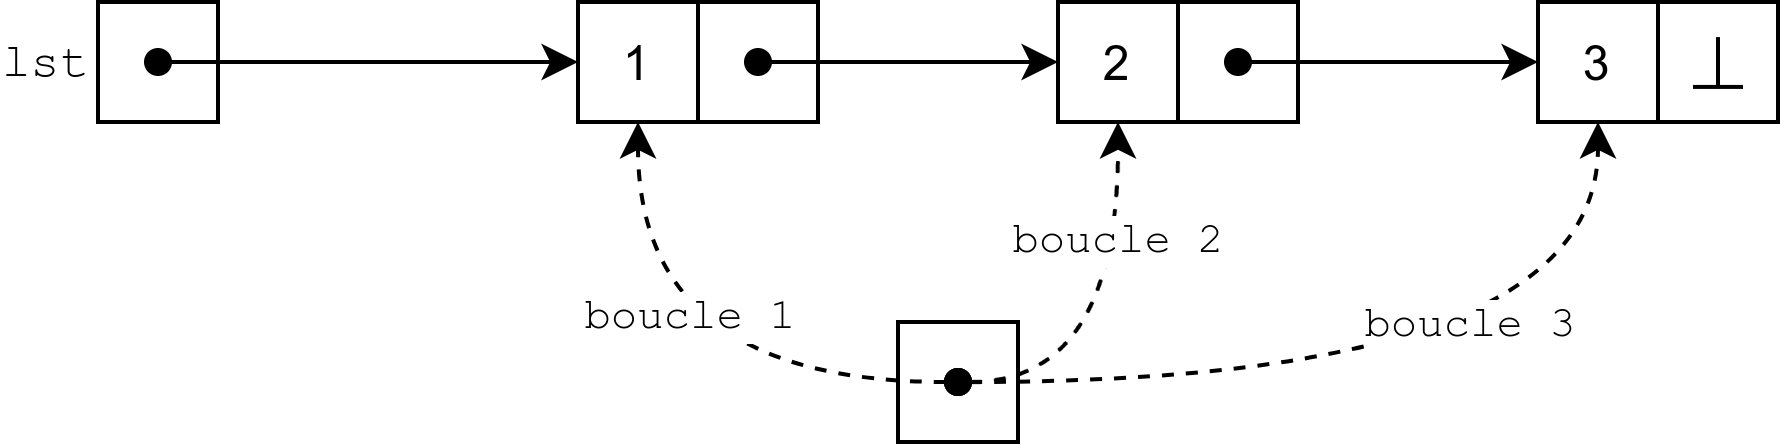
\includegraphics{maillon3.png}
\caption{algo récursif}
\end{figure}

Puis tant que le maillon courant n'est pas \texttt{None}, il faut
incrémenter l'accumulateur de 1 et mettre à jour le maillon courant avec
le maillon suivant.

Lorsque le boucle s'arrête, c'est que le maillon courant est
\texttt{None} et donc tous les maillons ont été visités. Il faut alors
renvoyer l'accumulateur qui contient le nombre de maillons visités, qui
est égal à la longueur de la liste.

        \end{retenir}\begin{eleve}
    \textbf{Implémenter la fonction itérative
\texttt{longueur(lst)\ -\textgreater{}\ int} qui renvoie la longueur de
la liste \texttt{lst}.}

\emph{Exemple 1 : l'instruction
\texttt{print(\ longueur(Maillon(42,\ None))\ )} doit afficher
\texttt{1} car cette liste ne contient qu'un seul maillon.}

\begin{verbatim}
    >>> print( longueur(Maillon(42, None)) )
    1
\end{verbatim}

\emph{Exemple 2 : l'instruction \texttt{print(\ longueur(None)\ )} doit
afficher \texttt{0} car c'est la liste vide.}

\begin{verbatim}
    >>> print( longueur(None) )
    0
\end{verbatim}

\emph{Exemple 3 : l'instruction
\texttt{print(longueur(\ Maillon(1,\ Maillon(2,\ Maillon(3,\ None)))\ ))}
doit afficher \texttt{3}.}

\begin{verbatim}
    >>> print(longueur( Maillon(1, Maillon(2, Maillon(3, None))) ))
    3
\end{verbatim}
        
        \end{eleve}\begin{reponse}
        {\scriptsize
    \begin{tcolorbox}[breakable, size=fbox, boxrule=1pt, pad at break*=1mm,colback=cellbackground, colframe=cellborder]
\prompt{In}{incolor}{4}{\boxspacing}
\begin{Verbatim}[commandchars=\\\{\}]
\PY{k}{def} \PY{n+nf}{longueur}\PY{p}{(}\PY{n}{lst}\PY{p}{)}\PY{p}{:}
    \PY{l+s+sd}{\PYZdq{}\PYZdq{}\PYZdq{} longueur d\PYZsq{}une liste chaînée}
\PY{l+s+sd}{    }
\PY{l+s+sd}{    Exemples et tests:}
\PY{l+s+sd}{    \PYZgt{}\PYZgt{}\PYZgt{} lst = Maillon(42, None)}
\PY{l+s+sd}{    \PYZgt{}\PYZgt{}\PYZgt{} assert longueur(lst) == 1}

\PY{l+s+sd}{    \PYZgt{}\PYZgt{}\PYZgt{} lst = None}
\PY{l+s+sd}{    \PYZgt{}\PYZgt{}\PYZgt{} assert longueur(lst) == 0}

\PY{l+s+sd}{    \PYZgt{}\PYZgt{}\PYZgt{} lst = Maillon(1, Maillon(2, Maillon(3, None)))}
\PY{l+s+sd}{    \PYZgt{}\PYZgt{}\PYZgt{} assert longueur(lst) == 3}
\PY{l+s+sd}{    \PYZdq{}\PYZdq{}\PYZdq{}}
    \PY{n}{longueur\PYZus{}actuelle} \PY{o}{=} \PY{l+m+mi}{0}
    \PY{n}{maillon\PYZus{}actuel} \PY{o}{=} \PY{n}{lst}

    \PY{k}{while} \PY{n}{maillon\PYZus{}actuel} \PY{o+ow}{is} \PY{o+ow}{not} \PY{k+kc}{None}\PY{p}{:}
        \PY{n}{longueur\PYZus{}actuelle} \PY{o}{=} \PY{n}{longueur\PYZus{}actuelle} \PY{o}{+} \PY{l+m+mi}{1}
        \PY{n}{maillon\PYZus{}actuel} \PY{o}{=} \PY{n}{maillon\PYZus{}actuel}\PY{o}{.}\PY{n}{suivant}
    
    \PY{k}{return} \PY{n}{longueur\PYZus{}actuelle}


\PY{n}{testmod}\PY{p}{(}\PY{p}{)}


\PY{n+nb}{print}\PY{p}{(}\PY{n}{longueur}\PY{p}{(}\PY{n}{Maillon}\PY{p}{(}\PY{l+m+mi}{42}\PY{p}{,} \PY{k+kc}{None}\PY{p}{)}\PY{p}{)} \PY{p}{)}
\PY{n+nb}{print}\PY{p}{(}\PY{n}{longueur}\PY{p}{(}\PY{k+kc}{None}\PY{p}{)} \PY{p}{)}
\PY{n+nb}{print}\PY{p}{(}\PY{n}{longueur}\PY{p}{(} \PY{n}{Maillon}\PY{p}{(}\PY{l+m+mi}{1}\PY{p}{,} \PY{n}{Maillon}\PY{p}{(}\PY{l+m+mi}{2}\PY{p}{,} \PY{n}{Maillon}\PY{p}{(}\PY{l+m+mi}{3}\PY{p}{,} \PY{k+kc}{None}\PY{p}{)}\PY{p}{)}\PY{p}{)} \PY{p}{)}\PY{p}{)}
\end{Verbatim}
\end{tcolorbox}
    }

    \begin{Verbatim}[commandchars=\\\{\}]
1
0
3
    \end{Verbatim}

        \end{reponse}
    \hypertarget{niuxe8me-uxe9luxe9ment-dune-liste}{%
\subsubsection{3.2 --- Nième élément d'une
liste}\label{niuxe8me-uxe9luxe9ment-dune-liste}}

    Comme pour la fonction précédente, on peut implémenter une version
itérative et une version récursive de la fonction demandée\ldots{}
\begin{eleve}
    \textbf{Implémenter une version itérative de la fonction
\texttt{nieme\_element(n,\ lst)} qui renvoie le \(n\)-ième élément d'une
liste chaînée. Évidement on prend par convention que le premier élément
est désigné par \(n=0\).}

\emph{Exemple 1 :
\texttt{print(\ nieme\_element(1,\ Maillon(42,\ None))\ )} affiche
\texttt{IndexError} car la liste chaînée n'a qu'un seul maillon (à
l'indice \(0\)) et donc pas de maillons à l'indice \(1\).}

\begin{verbatim}
    >>> print( nieme_element(1, Maillon(42, None)) )
    Traceback (most recent call last):
    IndexError: index out of range
\end{verbatim}

\emph{Exemple 2 :
\texttt{print(\ nieme\_element(1,\ Maillon(1,\ Maillon(2,\ Maillon(3,\ None))))\ )}affiche
\texttt{2} car le maillon d'indice \texttt{1} contient la valeur
\texttt{2}.}

\begin{verbatim}
    >>> print( nieme_element(1, Maillon(1, Maillon(2, Maillon(3, None)))) )
    2
\end{verbatim}
        
        \end{eleve}\begin{reponse}
        {\scriptsize
    \begin{tcolorbox}[breakable, size=fbox, boxrule=1pt, pad at break*=1mm,colback=cellbackground, colframe=cellborder]
\prompt{In}{incolor}{5}{\boxspacing}
\begin{Verbatim}[commandchars=\\\{\}]
\PY{k}{def} \PY{n+nf}{nieme\PYZus{}element}\PY{p}{(}\PY{n}{n}\PY{p}{,} \PY{n}{lst}\PY{p}{)}\PY{p}{:}
    \PY{l+s+sd}{\PYZdq{}\PYZdq{}\PYZdq{} nieme element d\PYZsq{}une liste chaînée}
\PY{l+s+sd}{        version itérative}
\PY{l+s+sd}{    }
\PY{l+s+sd}{    Exemples et tests:}
\PY{l+s+sd}{    \PYZgt{}\PYZgt{}\PYZgt{} lst = Maillon(1, Maillon(2, Maillon(3, None)))}
\PY{l+s+sd}{    \PYZgt{}\PYZgt{}\PYZgt{} assert nieme\PYZus{}element(0, lst) == 1}
\PY{l+s+sd}{    \PYZgt{}\PYZgt{}\PYZgt{} assert nieme\PYZus{}element(1, lst) == 2}
\PY{l+s+sd}{    \PYZgt{}\PYZgt{}\PYZgt{} assert nieme\PYZus{}element(2, lst) == 3}

\PY{l+s+sd}{    \PYZgt{}\PYZgt{}\PYZgt{} nieme\PYZus{}element(3, lst)}
\PY{l+s+sd}{    Traceback (most recent call last):}
\PY{l+s+sd}{    IndexError: index out of range}
\PY{l+s+sd}{    \PYZdq{}\PYZdq{}\PYZdq{}}
    \PY{k}{if} \PY{n}{n} \PY{o}{\PYZgt{}}\PY{o}{=} \PY{n}{longueur}\PY{p}{(}\PY{n}{lst}\PY{p}{)}\PY{p}{:}
        \PY{k}{raise} \PY{n+ne}{IndexError}\PY{p}{(}\PY{l+s+s1}{\PYZsq{}}\PY{l+s+s1}{index out of range}\PY{l+s+s1}{\PYZsq{}}\PY{p}{)}

    \PY{n}{maillon\PYZus{}actuel} \PY{o}{=} \PY{n}{lst}
    \PY{k}{for} \PY{n}{\PYZus{}} \PY{o+ow}{in} \PY{n+nb}{range}\PY{p}{(}\PY{n}{n}\PY{p}{)}\PY{p}{:}
        \PY{n}{maillon\PYZus{}actuel} \PY{o}{=} \PY{n}{maillon\PYZus{}actuel}\PY{o}{.}\PY{n}{suivant}
    \PY{k}{return} \PY{n}{maillon\PYZus{}actuel}\PY{o}{.}\PY{n}{valeur}


\PY{n}{testmod}\PY{p}{(}\PY{p}{)}
\end{Verbatim}
\end{tcolorbox}
    }

            \begin{tcolorbox}[breakable, size=fbox, boxrule=.5pt, pad at break*=1mm, opacityfill=0]
\prompt{Out}{outcolor}{5}{\boxspacing}
\begin{Verbatim}[commandchars=\\\{\}]
TestResults(failed=0, attempted=23)
\end{Verbatim}
\end{tcolorbox}
        
        \end{reponse}\begin{eleve}
    \textbf{Implémenter une version récursive de la fonction
\texttt{nieme\_element(n,\ lst)} qui renvoie le \(n\)-ième élément d'une
liste chaînée. Évidement on prend par convention que le premier élément
est désigné par \(n=0\).}

\emph{Exemple 1 :
\texttt{print(\ nieme\_element(1,\ Maillon(42,\ None))\ )} affiche
\texttt{IndexError} car la liste chaînée n'a qu'un seul maillon (à
l'indice \(0\)) et donc pas de maillons à l'indice \(1\).}

\begin{verbatim}
    >>> print( nieme_element(1, Maillon(42, None)) )
    IndexError
\end{verbatim}

\emph{Exemple 2 :
\texttt{print(\ nieme\_element.(1,\ Maillon(1,\ Maillon(2,\ Maillon(3,\ None))))\ )}affiche
\texttt{2} car le maillon d'indice \texttt{1} contient la valeur
\texttt{2}.}

\begin{verbatim}
    >>> print( nieme_element.(1, Maillon(1, Maillon(2, Maillon(3, None)))) )
    2
\end{verbatim}
        
        \end{eleve}\begin{reponse}
        {\scriptsize
    \begin{tcolorbox}[breakable, size=fbox, boxrule=1pt, pad at break*=1mm,colback=cellbackground, colframe=cellborder]
\prompt{In}{incolor}{6}{\boxspacing}
\begin{Verbatim}[commandchars=\\\{\}]
\PY{k}{def} \PY{n+nf}{nieme\PYZus{}element}\PY{p}{(}\PY{n}{n}\PY{p}{,} \PY{n}{lst}\PY{p}{)}\PY{p}{:}
    \PY{l+s+sd}{\PYZdq{}\PYZdq{}\PYZdq{} nieme element d\PYZsq{}une liste chaînée}
\PY{l+s+sd}{        version itérative}
\PY{l+s+sd}{    }
\PY{l+s+sd}{    Exemples et tests:}
\PY{l+s+sd}{    \PYZgt{}\PYZgt{}\PYZgt{} lst = Maillon(1, Maillon(2, Maillon(3, None)))}
\PY{l+s+sd}{    \PYZgt{}\PYZgt{}\PYZgt{} assert nieme\PYZus{}element(0, lst) == 1}
\PY{l+s+sd}{    \PYZgt{}\PYZgt{}\PYZgt{} assert nieme\PYZus{}element(1, lst) == 2}
\PY{l+s+sd}{    \PYZgt{}\PYZgt{}\PYZgt{} assert nieme\PYZus{}element(2, lst) == 3}

\PY{l+s+sd}{    \PYZgt{}\PYZgt{}\PYZgt{} assert nieme\PYZus{}element(3, lst) == 3}
\PY{l+s+sd}{    Traceback (most recent call last):}
\PY{l+s+sd}{    IndexError: index out of range}
\PY{l+s+sd}{    \PYZdq{}\PYZdq{}\PYZdq{}}
    \PY{k}{if} \PY{n}{n} \PY{o}{\PYZgt{}}\PY{o}{=} \PY{n}{longueur}\PY{p}{(}\PY{n}{lst}\PY{p}{)}\PY{p}{:}
        \PY{k}{raise} \PY{n+ne}{IndexError}\PY{p}{(}\PY{l+s+s1}{\PYZsq{}}\PY{l+s+s1}{index out of range}\PY{l+s+s1}{\PYZsq{}}\PY{p}{)}

    \PY{k}{if} \PY{n}{n} \PY{o}{==} \PY{l+m+mi}{0}\PY{p}{:}
        \PY{k}{return} \PY{n}{lst}\PY{o}{.}\PY{n}{valeur}

    \PY{k}{return} \PY{n}{nieme\PYZus{}element}\PY{p}{(}\PY{n}{n} \PY{o}{\PYZhy{}} \PY{l+m+mi}{1}\PY{p}{,} \PY{n}{lst}\PY{o}{.}\PY{n}{suivant}\PY{p}{)}


\PY{n}{testmod}\PY{p}{(}\PY{p}{)}
\end{Verbatim}
\end{tcolorbox}
    }

            \begin{tcolorbox}[breakable, size=fbox, boxrule=.5pt, pad at break*=1mm, opacityfill=0]
\prompt{Out}{outcolor}{6}{\boxspacing}
\begin{Verbatim}[commandchars=\\\{\}]
TestResults(failed=0, attempted=23)
\end{Verbatim}
\end{tcolorbox}
        
        \end{reponse}
    \hypertarget{concatuxe9nation-de-deux-listes}{%
\subsubsection{3.3 --- Concaténation de deux
listes}\label{concatuxe9nation-de-deux-listes}}

    Considérons maintenant l'opération consistant à mettre bout à bout les
éléments de deux listes données. On appelle cela la
\textbf{concaténation} de deux listes. Ainsi, si la première liste
contient 1,2,3 et la seconde 4,5 alors le résultat de la concaténation
est la liste 1,2,3,4,5.

Nous choisissons d'écrire la concaténation sous la forme d'une fonction
\texttt{concatener(l1,\ l2)} qui reçoit deux listes en arguments et
renvoie une troisième liste contenant la concaténation.
\begin{retenir}
    L'algorithme \textbf{récursif} est très simple :

\begin{itemize}
\tightlist
\item
  si la liste \texttt{l1} est vide, la concaténation est identique à
  \texttt{l2} et il suffit de renvoyer \texttt{l2}
\item
  sinon, le premier élément de la concaténation est le premier élément
  de \texttt{l1} et le reste de la concaténation est obtenu
  récursivement en concaténant le reste de \texttt{l1} avec \texttt{l2}.
\end{itemize}

        \end{retenir}\begin{eleve}
    \textbf{Implémenter la version récursive de la fonction
\texttt{concatener} qui prend deux listes \texttt{l1} et \texttt{l2} en
argument et renvoie la concaténation des deux listes.}

Exemples et tests:

\begin{verbatim}
    >>> l1 = Maillon(1, Maillon(2, Maillon(3, None)))
    >>> l2 = Maillon(4, Maillon(5, None))
    >>> l3 = concatener(l1, l2)
    >>> assert nieme_element(0, l3) == 1
    >>> assert nieme_element(1, l3) == 2
    >>> assert nieme_element(2, l3) == 3
    >>> assert nieme_element(3, l3) == 4
    >>> assert nieme_element(4, l3) == 5

    >>> nieme_element(5, l3)
    Traceback (most recent call last):
    IndexError: index out of range
\end{verbatim}
        
        \end{eleve}\begin{reponse}
        {\scriptsize
    \begin{tcolorbox}[breakable, size=fbox, boxrule=1pt, pad at break*=1mm,colback=cellbackground, colframe=cellborder]
\prompt{In}{incolor}{7}{\boxspacing}
\begin{Verbatim}[commandchars=\\\{\}]
\PY{k}{def} \PY{n+nf}{concatener}\PY{p}{(}\PY{n}{start\PYZus{}lst}\PY{p}{,} \PY{n}{end\PYZus{}lst}\PY{p}{)}\PY{p}{:}
    \PY{l+s+sd}{\PYZdq{}\PYZdq{}\PYZdq{} concaténer deux liste de façon récursive}
\PY{l+s+sd}{    }
\PY{l+s+sd}{    Exemples et tests:}
\PY{l+s+sd}{    \PYZgt{}\PYZgt{}\PYZgt{} l1 = Maillon(1, Maillon(2, Maillon(3, None)))}
\PY{l+s+sd}{    \PYZgt{}\PYZgt{}\PYZgt{} l2 = Maillon(4, Maillon(5, None))}
\PY{l+s+sd}{    \PYZgt{}\PYZgt{}\PYZgt{} l3 = concatener(l1, l2)}
\PY{l+s+sd}{    \PYZgt{}\PYZgt{}\PYZgt{} assert nieme\PYZus{}element(0, l3) == 1}
\PY{l+s+sd}{    \PYZgt{}\PYZgt{}\PYZgt{} assert nieme\PYZus{}element(1, l3) == 2}
\PY{l+s+sd}{    \PYZgt{}\PYZgt{}\PYZgt{} assert nieme\PYZus{}element(2, l3) == 3}
\PY{l+s+sd}{    \PYZgt{}\PYZgt{}\PYZgt{} assert nieme\PYZus{}element(3, l3) == 4}
\PY{l+s+sd}{    \PYZgt{}\PYZgt{}\PYZgt{} assert nieme\PYZus{}element(4, l3) == 5}

\PY{l+s+sd}{    \PYZgt{}\PYZgt{}\PYZgt{} nieme\PYZus{}element(5, l3)}
\PY{l+s+sd}{    Traceback (most recent call last):}
\PY{l+s+sd}{    IndexError: index out of range}

\PY{l+s+sd}{    \PYZdq{}\PYZdq{}\PYZdq{}}
    \PY{k}{if} \PY{n}{longueur}\PY{p}{(}\PY{n}{start\PYZus{}lst}\PY{p}{)} \PY{o}{==} \PY{l+m+mi}{0}\PY{p}{:}
        \PY{k}{return} \PY{n}{end\PYZus{}lst}

    \PY{n}{premier\PYZus{}element} \PY{o}{=} \PY{n}{Maillon}\PY{p}{(}\PY{n}{start\PYZus{}lst}\PY{o}{.}\PY{n}{valeur}\PY{p}{,} \PY{k+kc}{None}\PY{p}{)}
    \PY{n}{reste} \PY{o}{=} \PY{n}{concatener}\PY{p}{(}\PY{n}{start\PYZus{}lst}\PY{o}{.}\PY{n}{suivant}\PY{p}{,} \PY{n}{end\PYZus{}lst}\PY{p}{)}
    \PY{n}{premier\PYZus{}element}\PY{o}{.}\PY{n}{suivant} \PY{o}{=} \PY{n}{reste}
    \PY{k}{return} \PY{n}{premier\PYZus{}element}


\PY{n}{testmod}\PY{p}{(}\PY{p}{)}
\end{Verbatim}
\end{tcolorbox}
    }

            \begin{tcolorbox}[breakable, size=fbox, boxrule=.5pt, pad at break*=1mm, opacityfill=0]
\prompt{Out}{outcolor}{7}{\boxspacing}
\begin{Verbatim}[commandchars=\\\{\}]
TestResults(failed=0, attempted=32)
\end{Verbatim}
\end{tcolorbox}
        
        \end{reponse}\begin{remarque}
    Il est important de comprendre ici que les listes passées en argument à
la fonction concatener ne sont pas modifiées. Plus précisément, les
éléments de la liste \texttt{l1} sont copiés et ceux de \texttt{12} sont
partagés. Illustrons-le avec la concaténation des listes 1, 2, 3 et 4,
5. Après les trois instructions

\begin{Shaded}
\begin{Highlighting}[]
\NormalTok{l1 }\OperatorTok{=}\NormalTok{ Maillon(}\DecValTok{1}\NormalTok{, Maillon(}\DecValTok{2}\NormalTok{, Maillon(}\DecValTok{3}\NormalTok{, }\VariableTok{None}\NormalTok{)))}
\NormalTok{l2 }\OperatorTok{=}\NormalTok{ Maillon(}\DecValTok{4}\NormalTok{, Maillon(}\DecValTok{5}\NormalTok{, }\VariableTok{None}\NormalTok{))}
\NormalTok{l3 }\OperatorTok{=}\NormalTok{ concatener(l1, l2)}
\end{Highlighting}
\end{Shaded}

on a la situation suivante avec 8 maillons au total :

\begin{figure}
\centering
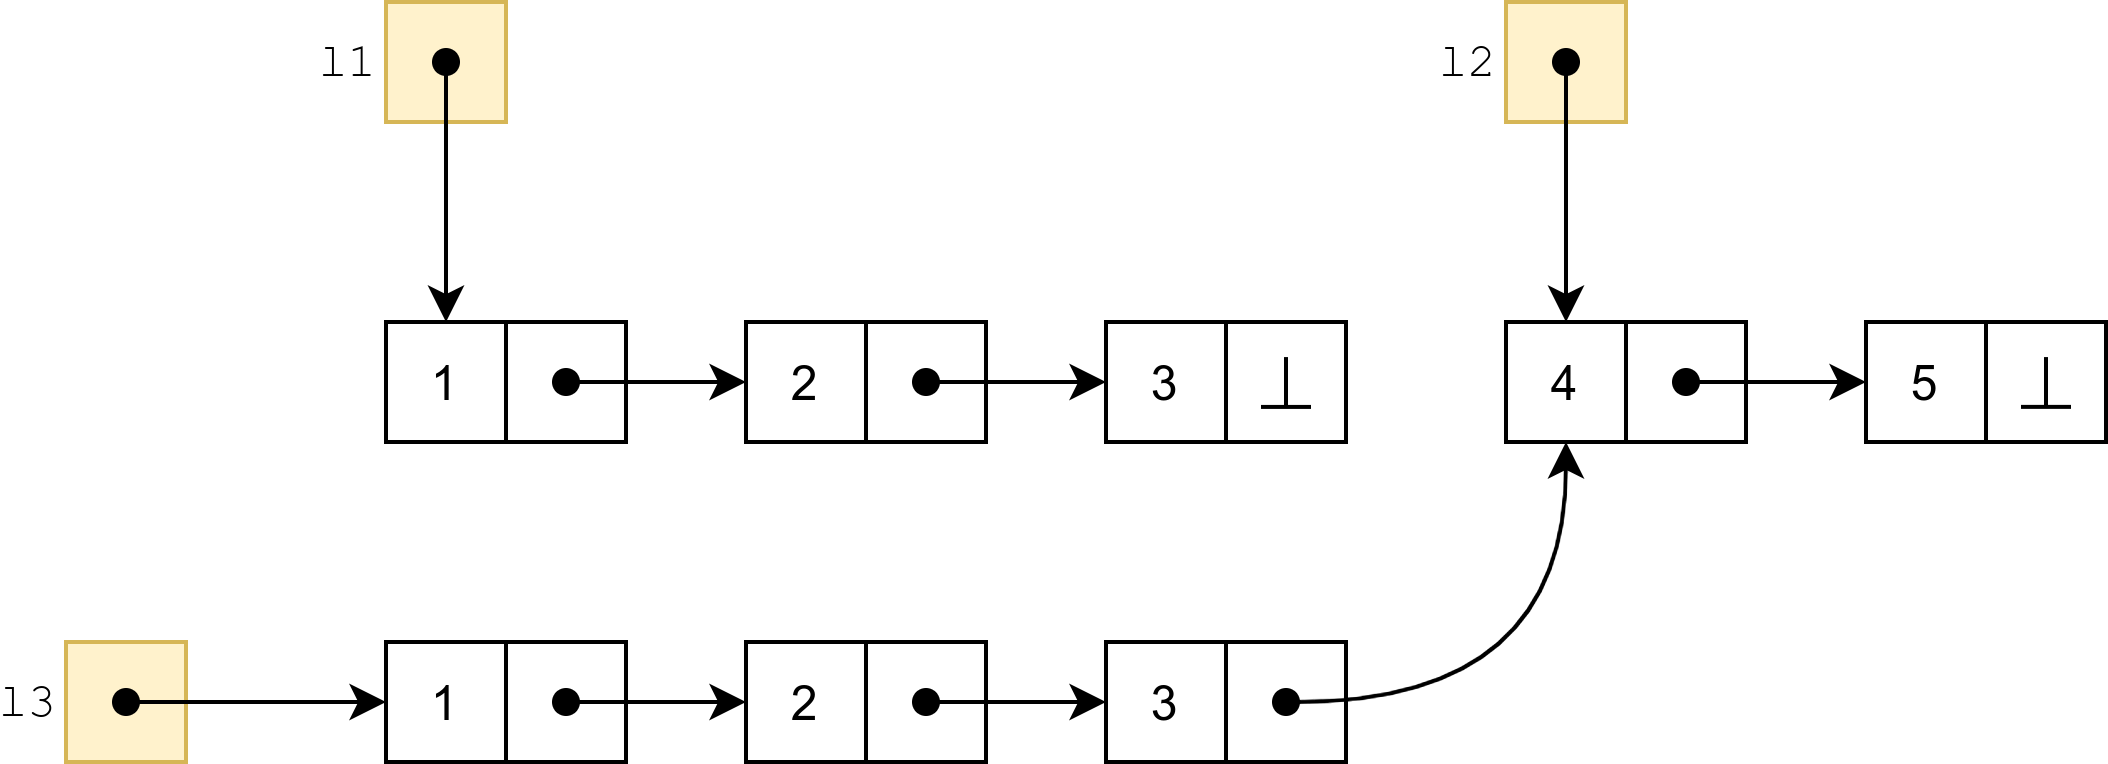
\includegraphics{maillon4.png}
\caption{concaténation de deux listes}
\end{figure}

        \end{remarque}
    \hypertarget{renverser-une-liste}{%
\subsubsection{3.4 --- Renverser une liste}\label{renverser-une-liste}}
\begin{eleve}
    \textbf{Implémenter une fonction \texttt{renverser(lst)} qui reçoit en
argument une liste comme 1, 2, 3 et renvoie la liste renversée 3, 2, 1.}

Exemples et tests:

\begin{verbatim}
    >>> l1 = Maillon(1, Maillon(2, Maillon(3, None)))
    >>> l2 = renverser(l1)
    >>> assert nieme_element(0, l2) == 3
    >>> assert nieme_element(1, l2) == 2
    >>> assert nieme_element(2, l2) == 1

    >>> nieme_element(3, l2)
    Traceback (most recent call last):
    IndexError: index out of range
\end{verbatim}
        
        \end{eleve}\begin{reponse}
        {\scriptsize
    \begin{tcolorbox}[breakable, size=fbox, boxrule=1pt, pad at break*=1mm,colback=cellbackground, colframe=cellborder]
\prompt{In}{incolor}{8}{\boxspacing}
\begin{Verbatim}[commandchars=\\\{\}]
\PY{k}{def} \PY{n+nf}{renverser}\PY{p}{(}\PY{n}{lst}\PY{p}{)}\PY{p}{:}
    \PY{l+s+sd}{\PYZdq{}\PYZdq{}\PYZdq{} renvoyer une nouvelle liste chainée renversée}
\PY{l+s+sd}{    }
\PY{l+s+sd}{    Exemples et tests:}
\PY{l+s+sd}{    \PYZgt{}\PYZgt{}\PYZgt{} l1 = Maillon(1, Maillon(2, Maillon(3, None)))}
\PY{l+s+sd}{    \PYZgt{}\PYZgt{}\PYZgt{} l2 = renverser(l1)}
\PY{l+s+sd}{    \PYZgt{}\PYZgt{}\PYZgt{} assert nieme\PYZus{}element(0, l2) == 3}
\PY{l+s+sd}{    \PYZgt{}\PYZgt{}\PYZgt{} assert nieme\PYZus{}element(1, l2) == 2}
\PY{l+s+sd}{    \PYZgt{}\PYZgt{}\PYZgt{} assert nieme\PYZus{}element(2, l2) == 1}

\PY{l+s+sd}{    \PYZgt{}\PYZgt{}\PYZgt{} nieme\PYZus{}element(3, l2)}
\PY{l+s+sd}{    Traceback (most recent call last):}
\PY{l+s+sd}{    IndexError: index out of range}
\PY{l+s+sd}{    \PYZdq{}\PYZdq{}\PYZdq{}}
    \PY{n}{n} \PY{o}{=} \PY{n}{longueur}\PY{p}{(}\PY{n}{lst}\PY{p}{)}
    \PY{n}{new\PYZus{}lst} \PY{o}{=} \PY{k+kc}{None}
    \PY{k}{for} \PY{n}{i} \PY{o+ow}{in} \PY{n+nb}{range}\PY{p}{(}\PY{n}{n}\PY{p}{)}\PY{p}{:}
        \PY{n}{valeur} \PY{o}{=} \PY{n}{nieme\PYZus{}element}\PY{p}{(}\PY{n}{i}\PY{p}{,} \PY{n}{lst}\PY{p}{)}
        \PY{n}{new\PYZus{}lst} \PY{o}{=} \PY{n}{Maillon}\PY{p}{(}\PY{n}{valeur}\PY{p}{,} \PY{n}{new\PYZus{}lst}\PY{p}{)}
    \PY{k}{return} \PY{n}{new\PYZus{}lst}


\PY{n}{testmod}\PY{p}{(}\PY{p}{)}
\end{Verbatim}
\end{tcolorbox}
    }

            \begin{tcolorbox}[breakable, size=fbox, boxrule=.5pt, pad at break*=1mm, opacityfill=0]
\prompt{Out}{outcolor}{8}{\boxspacing}
\begin{Verbatim}[commandchars=\\\{\}]
TestResults(failed=0, attempted=38)
\end{Verbatim}
\end{tcolorbox}
        
        \end{reponse}

    % Add a bibliography block to the postdoc
    
    
    
\end{document}
